\documentclass[14pt]{extarticle}

\usepackage{fontspec}
\setmainfont{Times New Roman}

% размер полей
\usepackage{geometry}
\geometry{a4paper, top=2cm, bottom=2cm, right=1.5cm, left=3cm}

 %debugging
%\usepackage{showframe}

% полуторный интервал
\usepackage{setspace}
\onehalfspacing

% абзацный отступ
\setlength{\parindent}{1.25cm}

% выравнивание текста по ширине
\sloppy

% списки
\usepackage{calc} % арифметические операции с величинами
\usepackage{enumitem}
\setlist{
    nosep,
    leftmargin=0pt,
    itemindent=\parindent + \labelwidth - \labelsep,
}

% подписи к рисункам и таблицам
\usepackage{caption}
\renewcommand{\figurename}{Рисунок}
\renewcommand{\tablename}{Таблица}
\DeclareCaptionFormat{custom}
{
    \textit{#1#2#3}
}
\DeclareCaptionLabelSeparator{custom}{. }
\captionsetup{
    % хз какой это размер - 12 или нет, но выглядит меньше 14
    font=small,
    format=custom,
    labelsep=custom,
}

% картинки
\usepackage{graphicx}

% колонтитулы
\usepackage{fancyhdr}

% картинки и таблицы находятся именно в том месте текста где помещены (атрибут H)
\usepackage{float}

% таблицы
\usepackage{tabularray}

\graphicspath{ {8.2.1/models/} }
\usepackage{hyperref}
\begin{document}
\pagestyle{fancy}
\fancyhead{}
% disable header
\renewcommand{\headrulewidth}{0pt}
\fancyfoot[L]{Дубровских гр 221-361}
\fancyfoot[C]{ЛР 8.2.1}
\fancyfoot[R]{Продажа автотранспорта}
\singlespacing

\newpage
\begin{center}
    Министерство науки и высшего образования Российской Федерации
    Федеральное государственное автономное образовательное учреждение

    высшего образования

    \guillemotleft МОСКОВСКИЙ ПОЛИТЕХНИЧЕСКИЙ УНИВЕРСИТЕТ\guillemotright

    (МОСКОВСКИЙ ПОЛИТЕХ)
\end{center}
\noindent
\bigbreak
\bigbreak
\bigbreak
\bigbreak
\begin{center}
    ЛАБОРАТОРНАЯ РАБОТА 8.2.1

    По курсу Проектирования пользовательских интерфейсов в веб

    \textbf{Создание основных страниц (прототипов страниц) в программном ресурсе.Использование Гайдлайнов и UI- Kit}
    \bigbreak
    \bigbreak
    \bigbreak
    \bigbreak
    ТЕМА

    \guillemotleft\textbf{САЙТ ДЛЯ ПРОДАЖИ И ПОИСКА АВТОМОБИЛЕЙ}\guillemotright
\end{center}
\noindent
\bigbreak
\bigbreak
\bigbreak
\bigbreak
\bigbreak
\bigbreak
\bigbreak
\bigbreak
\bigbreak
\bigbreak
\hfill Выполнил

\hfill Дубровских Никита Евгеньевич

\hfill Группа 221-361
\bigbreak
\bigbreak
\bigbreak
\hfill Проверил

\hfill Натур ВВ
\vfill
\begin{center}
    Москва, 2024
\end{center}
\newpage
\onehalfspacing


\begin{center}
    \textbf{Лабораторная работа 8.2.1}

    \textbf{Создание основных страниц (прототипов страниц) в программном ресурсе.Использование Гайдлайнов и UI- Kit}
\end{center}

\textbf{Цель работы:} разработать макеты демонстрационных страниц для прототипа интерфейса веб-сайта (мобильного приложения)
\bigskip

\textbf{Задачи:}

\begin{enumerate}
    \item Используя принципы «атомарного дизайна», разработать все необходимые компоненты страниц
    \item Познакомиться с Дизайн-системой - UI- KIT, фреймворки и гайдлайны
    \item Рассмотреть и применить при проектировании гайдлайны
    \item Рассмотреть и применить при проектировании UI- Kit
    \item Собрать страницы из компонентов и необходимых графических элементов по ранее разработанным вайрфреймам
\end{enumerate}
\bigskip

\textbf{Основные термины}

\begin{itemize}
    \item Атомарный дизайн — методология, в которой интерфейс разделяется на минимальные функциональные единицы (атомы), такие как кнопки, иконки, чекбоксы и т.д. Эти элементы собираются в более сложные компоненты (молекулы, организмы) и системы для создания интерфейсов.
    \item Компоненты в Figma — повторяющиеся элементы дизайна, которые можно использовать на нескольких страницах (например, шапка или подвал сайта). При изменении мастер-компонента все дочерние копии обновляются автоматически.
    \item UI-kit (набор интерфейсных элементов) — это готовый комплект графических элементов для пользовательского интерфейса, который можно использовать для создания страниц и экранов. Он помогает стандартизировать дизайн, экономит время и улучшает командное взаимодействие.
    \item Гайдлайны — набор правил и рекомендаций по дизайну интерфейсов, который определяет, как должны выглядеть и взаимодействовать элементы приложения. Примеры популярных гайдлайнов — Material Design (Google) и Human Interface Guidelines (Apple).
    \item Респонсивная верстка — адаптация дизайна для разных размеров экранов с использованием гибких сеток, изображений и CSS-медиа-запросов.
    \item Адаптивная верстка — использование нескольких фиксированных макетов для различных разрешений экранов.
\end{itemize}
\bigskip

\textbf{Гайдлайн и UI-кит}
\bigskip

В качестве гайдлайна и UI-кита был выбран Material Design 3:

\begin{table}[H]
    \small
    \setstretch{1}
    \begin{tabular}{|p{3cm}|p{5cm}|p{6cm}|}
\hline
\textbf{Компонент} & \textbf{Описание} & \textbf{Рекомендации} \\
\hline
Цвет & Цветовая палитра Material Design включает основные и акцентные цвета. & Используйте яркие, насыщенные цвета для акцентов, приглушенные для фона. Цвета должны быть доступными для всех пользователей. \\
\hline
Типографика & Material использует набор шрифтов, в основном Roboto и Noto. & Стремитесь к ясности и читаемости. Размеры шрифтов от 12 до 96 px для различных уровней иерархии. \\
\hline
Иконки & Простые, монотонные, легко читаемые иконки с четким значением. & Размер иконок от 18 до 48 dp. Используйте Material Icons или их аналоги. \\
\hline
Отступы и сетка & Сетка и отступы помогают организовать пространство, создавая гармоничную структуру. & Стандартный отступ — 8 dp. Сетки 4 и 8 dp обеспечивают аккуратное расположение элементов. \\
\hline
Карточки & Карточки группируют информацию и действия для отдельной темы. & Используйте тени и закругленные углы. Размеры иерархичны и зависят от контекста. \\
\hline
Кнопки & Кнопки используют понятные действия и предлагают кликать по ним. & Основные кнопки – акцентные цвета, а второстепенные – приглушенные. Закруглённые углы улучшают восприятие. \\
\hline
Анимация и переходы & Анимации добавляют интерактивности и помогают пользователям понять результаты своих действий. & Анимации должны быть короткими (до 300 мс) и поддерживать естественность движений. \\
\hline
Взаимодействие & Касания, жесты и поведение взаимодействий стандартизированы. & Минимальный размер для кликабельных областей – 48x48 dp. Жесты должны быть интуитивными. \\
\hline
Поверхности и слои & Система поверхностей основана на Z-оси, что помогает организовать слои информации. & Используйте тени и высоту для обозначения слоев, акцентируя важные элементы. \\
\hline
Состояния элементов & Состояния (нажато, наведено, отключено) помогают пользователям понять текущую доступность или состояние элементов интерфейса. & Обозначайте состояния с помощью цветов и тени. Отключенные элементы должны выглядеть приглушённо и быть неподвижны. \\
\hline
Форма элементов & Закругленные углы и плавные переходы делают интерфейс более дружественным и современным. & Рекомендуется закругление от 4 до 16 dp в зависимости от компонента. \\
\hline
\end{tabular}
\end{table}

\noindent
\begin{minipage}{\linewidth}
    \fbox{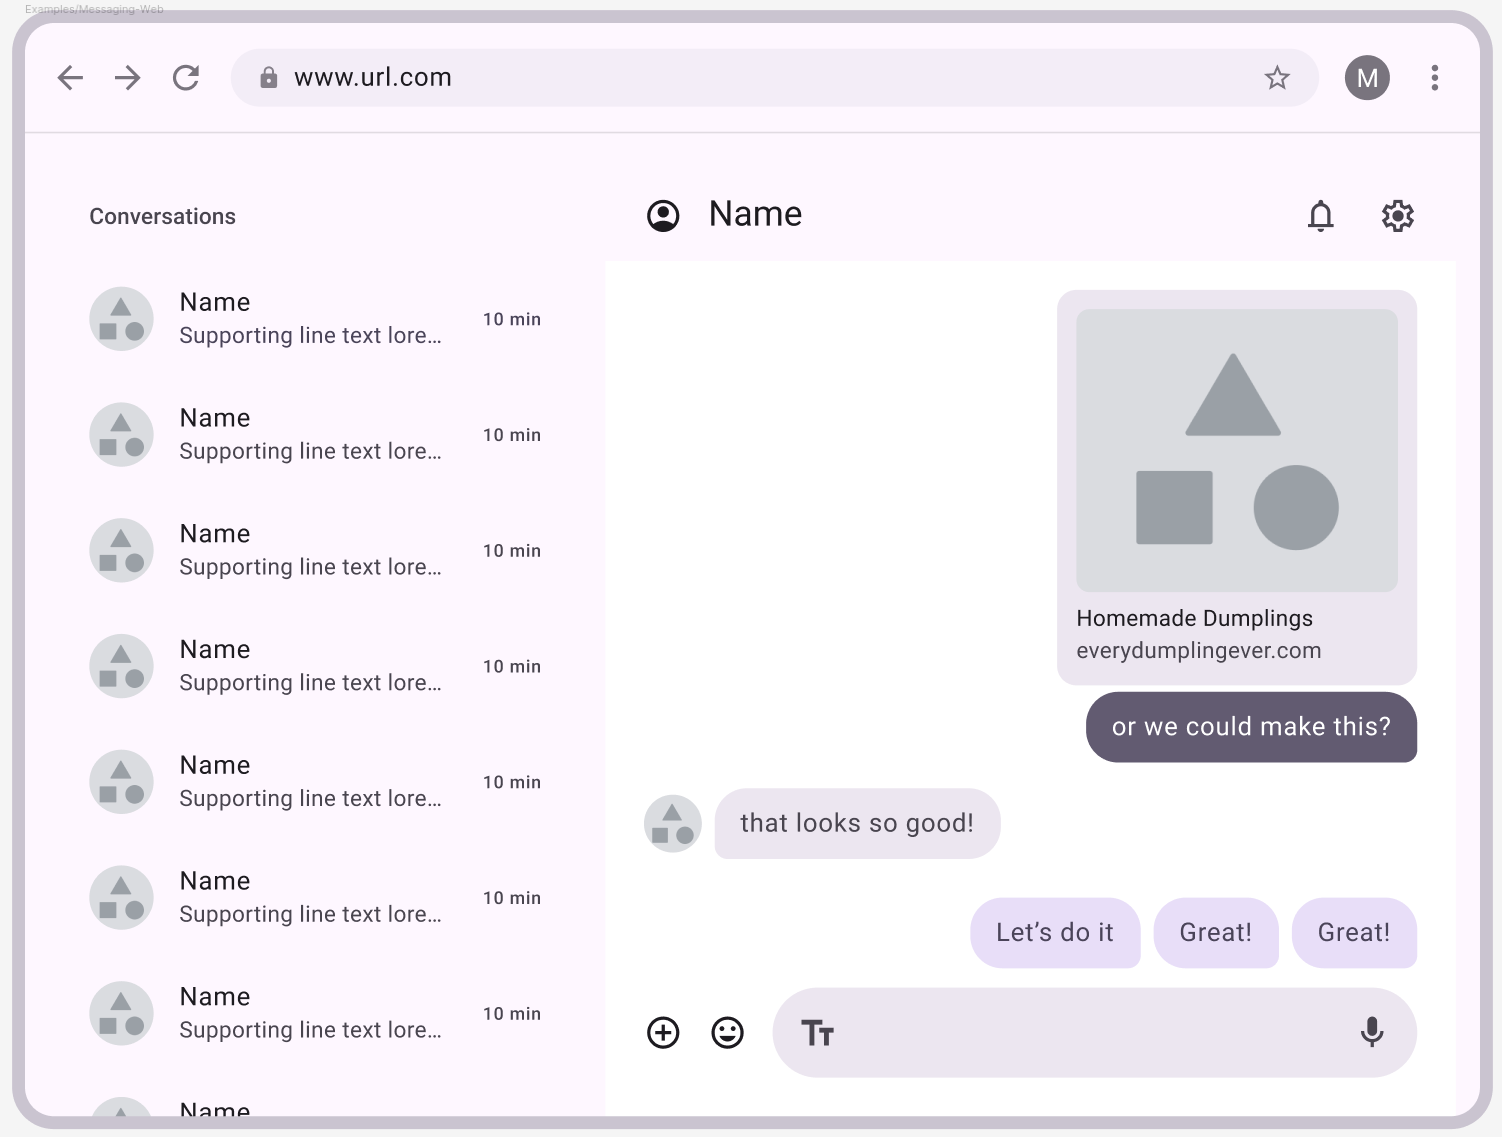
\includegraphics[width=\linewidth]{m3_1}}
\end{minipage}
\bigskip

\noindent
\begin{minipage}{\linewidth}
    \fbox{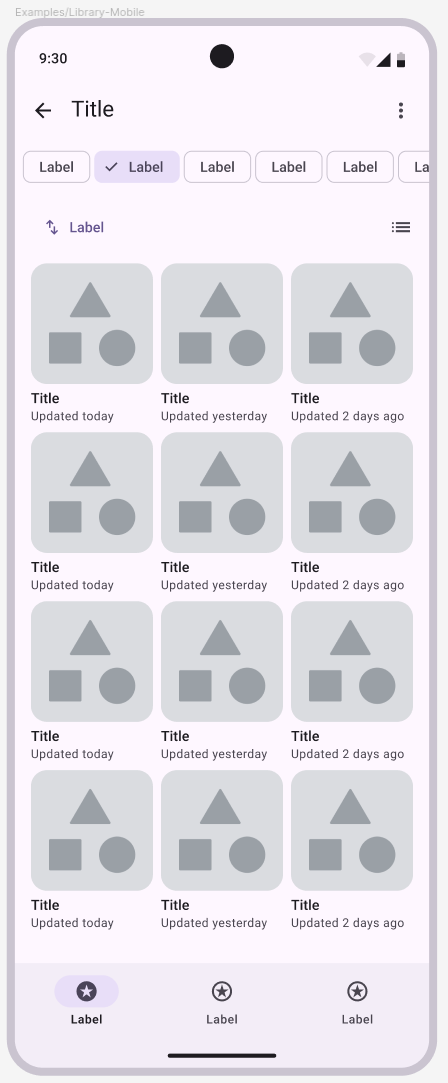
\includegraphics[scale=0.55]{m3_2}}
\end{minipage}
\bigskip

Ссылка:

\url{https://www.figma.com/community/file/1035203688168086460/material-3-design-kit}
\bigskip

\textbf{Прототипы}
\bigskip

\noindent
\begin{minipage}{\linewidth}
    \fbox{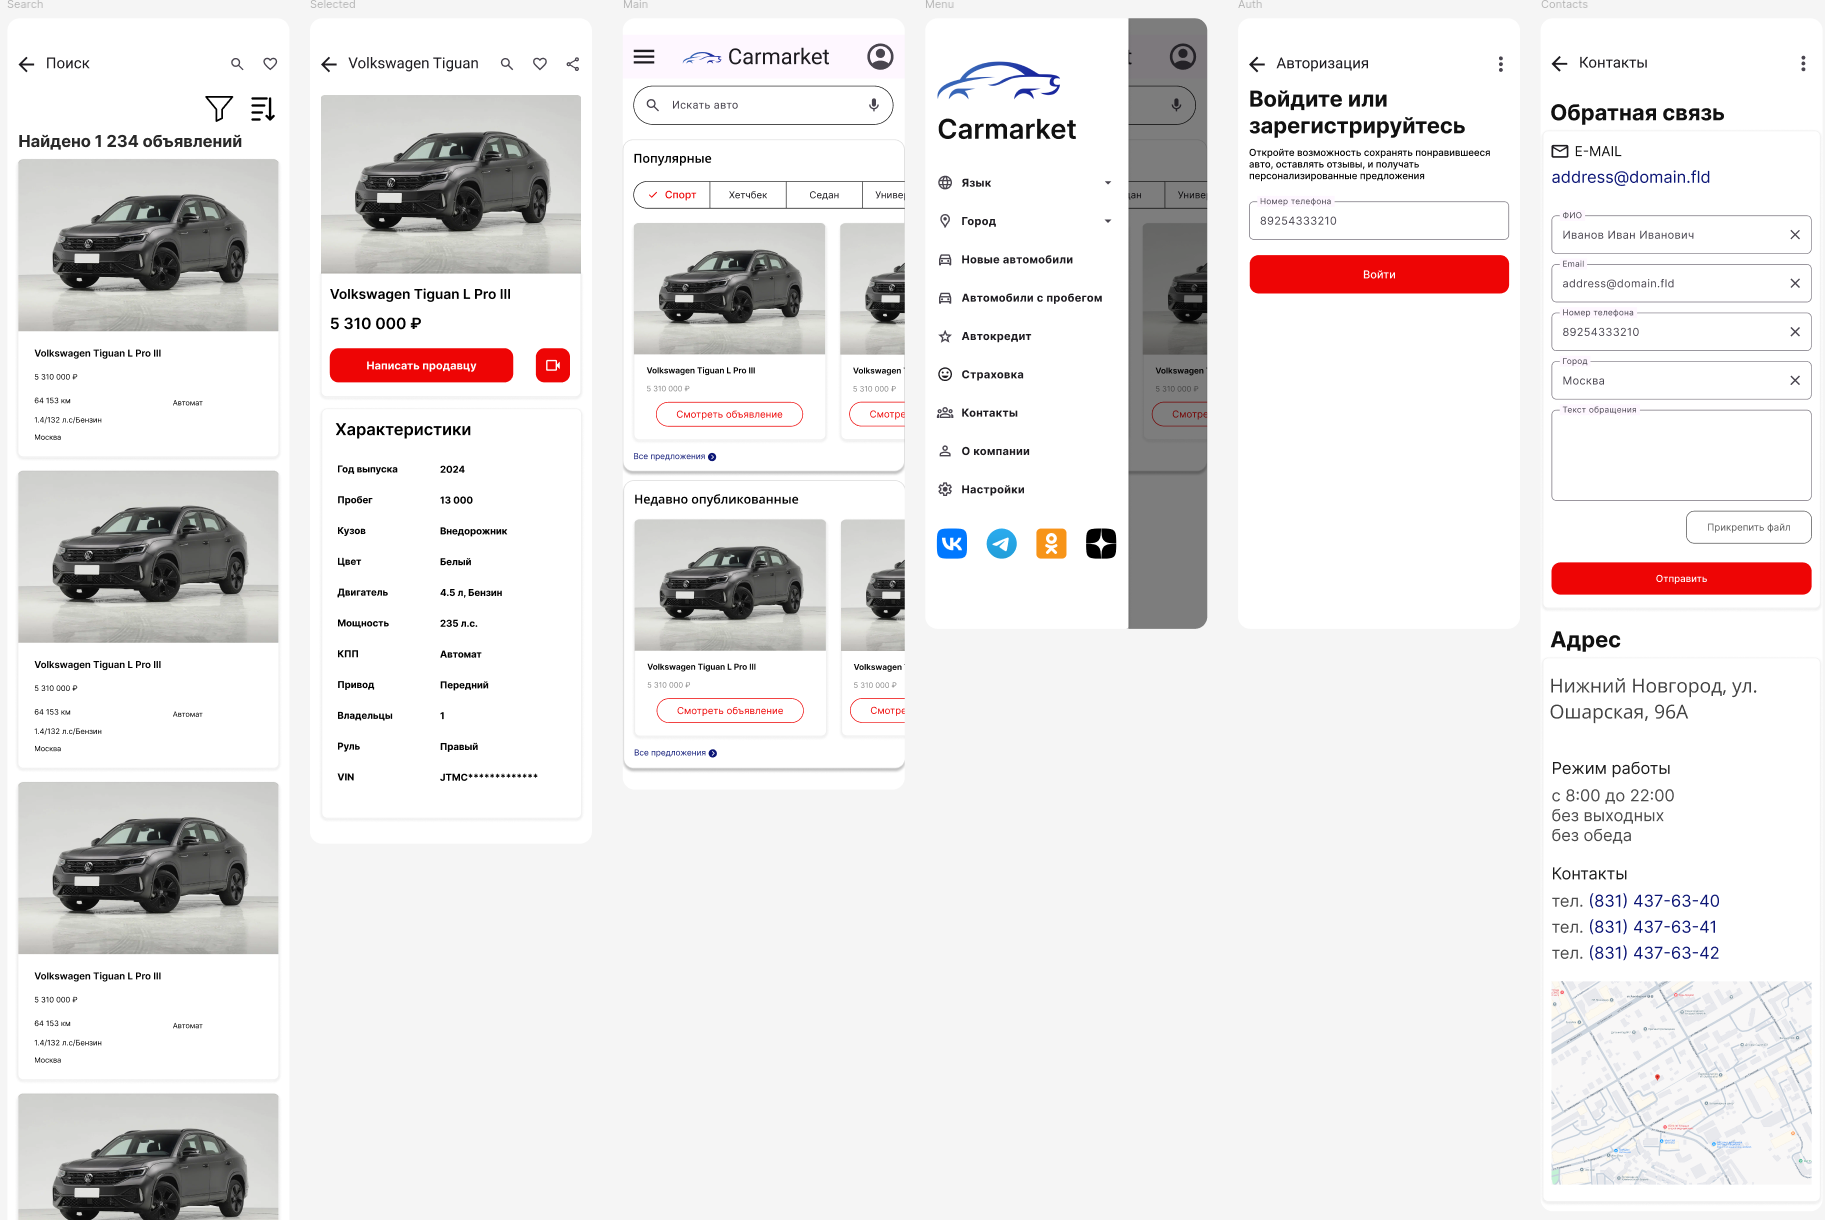
\includegraphics[width=\linewidth]{my1}}
\end{minipage}
\bigskip

\noindent
\begin{minipage}{\linewidth}
    \fbox{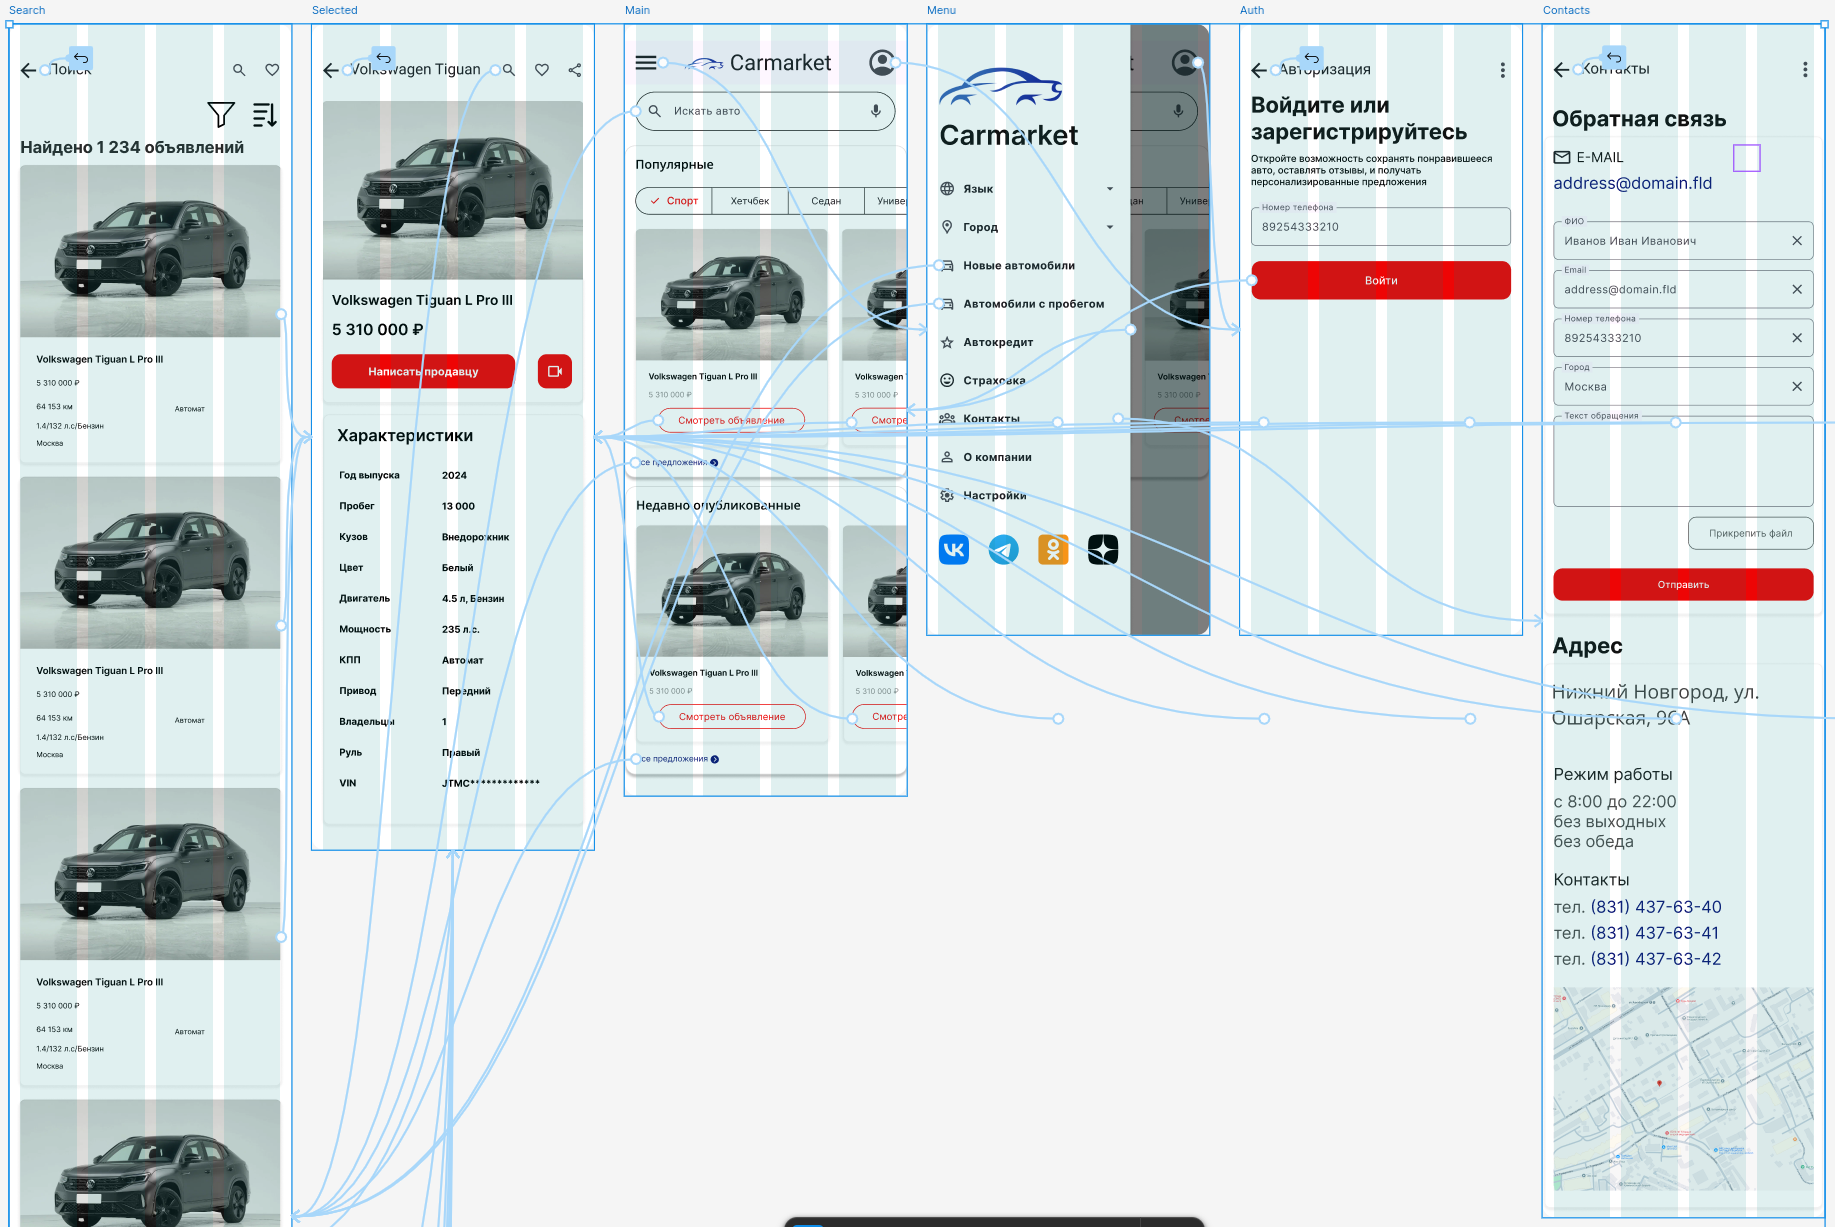
\includegraphics[width=\linewidth]{my2}}
\end{minipage}
\bigskip

\noindent
\begin{minipage}{\linewidth}
    \fbox{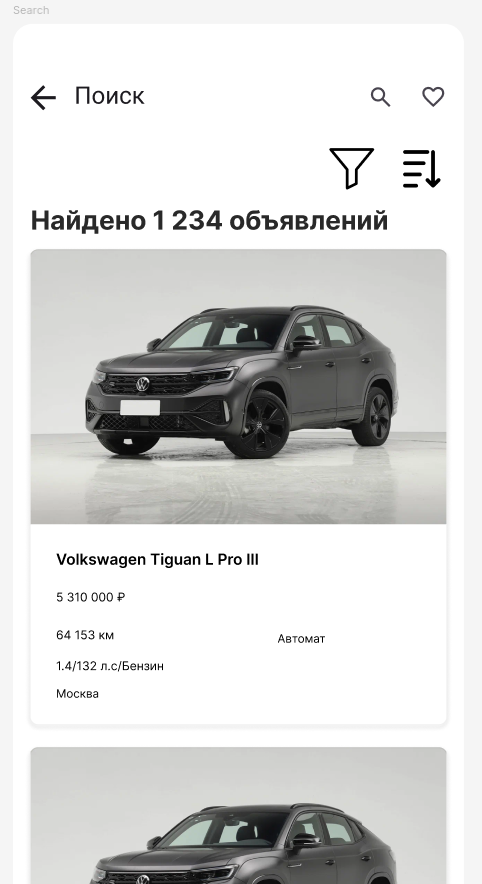
\includegraphics[width=\linewidth]{my3}}
\end{minipage}
\bigskip

\noindent
\begin{minipage}{\linewidth}
    \fbox{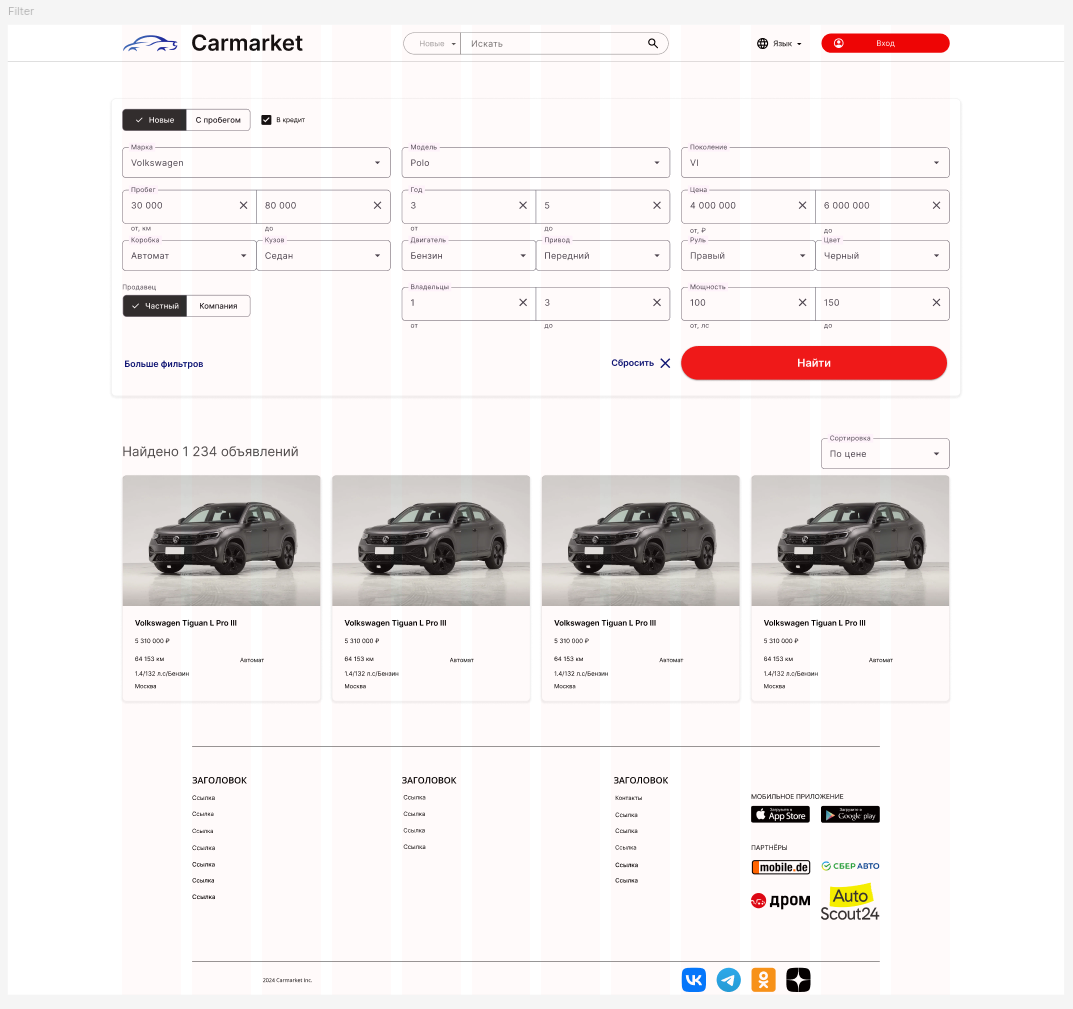
\includegraphics[width=\linewidth]{my4}}
\end{minipage}
\bigskip

\noindent
\begin{minipage}{\linewidth}
    \fbox{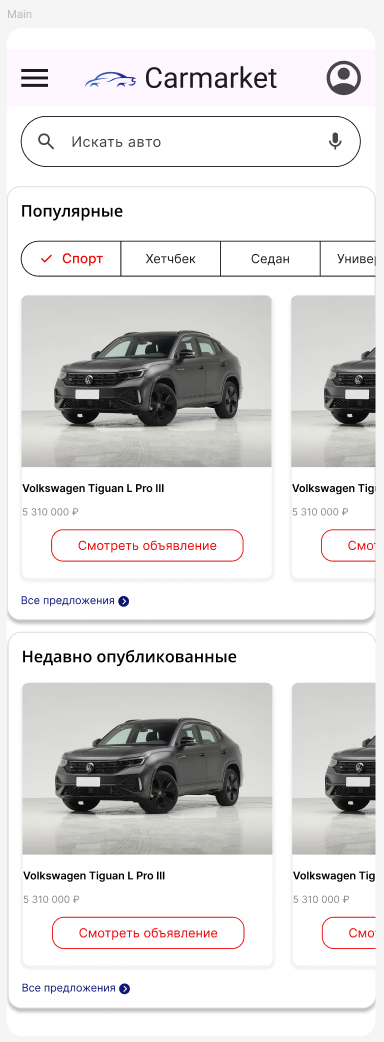
\includegraphics[width=\linewidth]{my5}}
\end{minipage}
\bigskip

Ссылка на Figma:

\url{https://www.figma.com/design/25STw8qqDFUKFnCIDQb1ri/PPI?node-id=0-1&t=3GTfYjQGpyVoN70i-1}
\bigskip

\textbf{Контрольные вопросы и ответы}

\begin{enumerate}
    \item Что такое атомарный дизайн веб-сайта?

    Атомарный дизайн — это методология создания интерфейсов, основанная на делении компонентов на более мелкие части. Она включает «атомы» (базовые элементы, такие как кнопки и ссылки), «молекулы» (группы элементов, которые работают вместе, как поле поиска), и «организмы» (большие группы элементов, например, шапка или карточка товара). Это помогает строить интерфейс системно и гибко, облегчая редактирование и стандартизацию.

\item Когда используются гайдлайны?

    Гайдлайны используются для обеспечения консистентности интерфейса и удобства взаимодействия пользователя с приложением или сайтом. Они предлагают стандарты, инструкции и рекомендации, как дизайн должен выглядеть и функционировать. Гайдлайны нужны для создания приложений, которые будут соответствовать требованиям платформ (например, Material Design для Android или HIG для iOS).

\item Когда используются UI-Kit?

    UI-Kit применяется при проектировании интерфейсов для ускорения процесса дизайна. Это набор готовых компонентов (кнопок, полей, иконок и пр.), которые можно использовать для сборки страниц или приложений. UI-Kit полезен для поддержания единого стиля и упрощения командной работы, поскольку все элементы собраны в одном месте и имеют стандартизированный вид.

\item Какие основные блоки входят в главную страницу?

        Шапку (логотип, меню навигации, контактные данные)

        Основной баннер или заголовок

        Преимущества или ключевые предложения

        Основной контент (новости, товары, статьи и т.п.)

        Футер (контакты, ссылки, политика конфиденциальности)

    \item В чем различие респонсивной и адаптивной верстки?

    Респонсивная верстка автоматически адаптирует интерфейс под любой экран за счет использования гибких сеток и элементов. Адаптивная верстка предполагает создание нескольких заранее определенных макетов под определенные размеры экранов, переключаясь между ними.

\item Рекомендации по выбору формата сайта:

    При выборе формата сайта необходимо учитывать целевую аудиторию и тип контента. Для сервисов и новостных сайтов важно выбрать респонсивный формат, чтобы контент адаптировался на любых устройствах. Для приложений с фиксированными требованиями можно использовать адаптивный формат с макетами для разных разрешений.


\end{enumerate}

\end{document}
